% !TeX TS-program = lualatex
% Based on work by Knsgf and brought to LaTeX by monabuu
% This work is distributed under the Unlicense (see LICENSE)
% SPDX-License-Identifier: Unlicense

% Compile with LuaLaTeX (TeX Live 2026)

\documentclass[11pt, a4paper]{article}
\usepackage{graphicx}
\usepackage[margin=2cm]{geometry}
\usepackage{xcolor}
\usepackage{array}
\usepackage{microtype}
\usepackage{fontspec}
\setmainfont{Liberation Sans}
\usepackage{parskip}
\usepackage{hyperref}
\hypersetup{colorlinks = true,
            linkcolor = blue}

% This sets up the pretty power mode and brake mode selector symbols. 
% The vertical alignment within a line of text may be adjusted by changing the value of the first argument of \raisebox.
\newcommand{\powermode}[1]{%
    \begingroup
    \setlength{\fboxsep}{0pt}%
    \raisebox{0.1em}{%
        \colorbox{black}{%
            \parbox[c][1.4em][c]{1.4em}{%
                \centering
                \color{white}\bfseries #1%
            }%
        }%
    }%
    \endgroup
}
\newcommand{\brakemode}[1]{%
    \begingroup
    \setlength{\fboxsep}{0pt}%
    \raisebox{0.1em}{%
        \colorbox{red}{%
            \parbox[c][1.4em][c]{1.4em}{%
                \centering
                \color{black}\bfseries #1%
            }%
        }%
    }%
    \endgroup
}

% Macros for recurring exclamations.
% Notice, that there is a choice to either inlcude a trailing space in the macro text or to add "\ " after macro usage to ensure correct spacing. I have chosen the latter but there is no reason apparent to me to go with one or the other.
\newcommand{\danger}{\textbf{\color{red} ! DANGER !}}
\newcommand{\caution}{\textbf{\color{orange} ! CAUTION !}}
\newcommand{\note}{\textbf{Note:}}
\newcommand{\NB}{\textbf{NB!}}
\newcommand{\Tip}{\textbf{Tip:}}

\begin{document}

\begin{titlepage}
    \centering
    \vspace*{1cm}
    {\Huge 2WE3 Operating Manual}
    \vspace{2cm}
    \tableofcontents
    \vfill
    This work is dedicated to the public under the \href{https://unlicense.org/}{Unlicense}
\end{titlepage}

\section{Short description}

The 2WE3 is a 6 axle DC B-B-B electric locomotive with resistance control, designed for heavy freight haulage on lines electrified with 1000-1500 V. The locomotive consists of 2 articulated units A and B, allowing it to operate in areas with high degrees of curvature.

\section{Technical specifications}

\begin{tabular}{@{}p{75mm}p{75mm}@{}}
Length & 2x11 m (72 ft)\\
Width & 3.2 m (10.5 ft)\\
Height above rail & 5.2 m (17 ft) with pantographs stowed\\
Contact wire height & \\
\hspace{15mm}minimum & 5.4 m (17.7 ft)\\
\hspace{15mm}maximum & 6.6 m (21.6 ft)\\
Weight & 170 metric tons (187 short tons)\\
Wheel arrangement & B-B-B (Bo'Bo'Bo')\\
Axle load & 28.3 metric tons/axle (62400 lbs/axle)\\
Driver diameter & 1120 mm (44 in)\\
Power supply & \\
\hspace{15mm}nominal & 1500 V DC,\\
\hspace{15mm}maximum & 2000 V,\\
\hspace{15mm}minimum permitted & 600 V\footnotemark\\
Continuous power output & 6x700 kW (5600 hp) at 1500 V\\
Continuous tractive effort & 300 kN (67000 lbf)\\
Continuous speed & 50 km/h (30 mph) at 1500 V\\
Maximum speed & 90 km/h (55 mph)\\
Braking systems & air, rheostatic, regenerative\\
Maximum continuous motor current & 500 A\\
Traction motor pole saturation current & 300 A\\
Continuous resistor power rating & 3 MW (4000 hp)\\
\end{tabular}
\footnotetext{Some systems, like air compressor and regenerative brake, will not run at minimum voltage.}
\newpage

\section{Locomotive systems and controls}

\subsection{Battery panel}
\begin{center}
 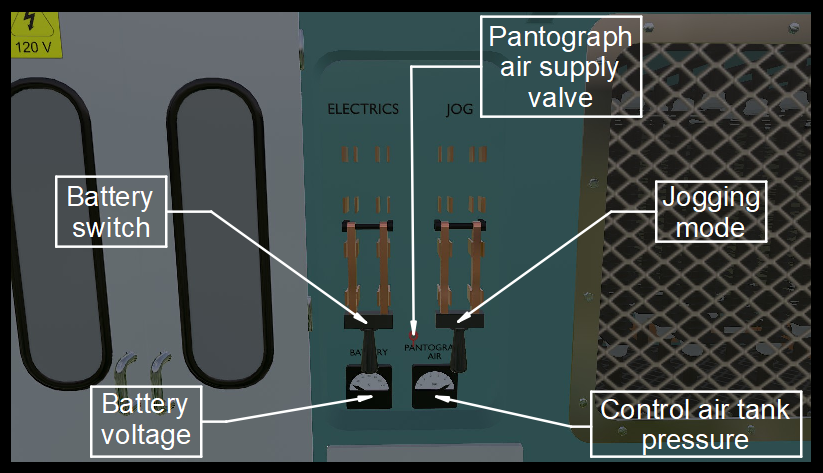
\includegraphics[width=\textwidth]{assets/img-000.png}
\end{center}
The battery panel, located in the machinery room of unit B, provides electrical and compressed air power for all onboard systems and installed gadgets. It includes ``Electrics'' and ``Jog'' knife switches, used to toggle onboard appliances and to move a locomotive around a roundhouse, respectively, and a ``Pantograph air'' valve, which supplies control air pressure to pantographs and switchgear. Switching off the ``Electrics'' or closing the ``Pantograph air'' valve will immediately retract all pantographs.

At the bottom of the panel there are two gauges: the left shows battery voltage, the right displays pressure in a dedicated control air tank. The locomotive requires at least 3 bar in the tank to run. The tank is replenished from main air reservoirs via a check valve; in the event of main reservoir lacking sufficient air there is a small auxiliary compressor, which automatically pumps control air to 4 bar.
\newpage

\subsection{Cab controls, switches and indicators}
\begin{center}
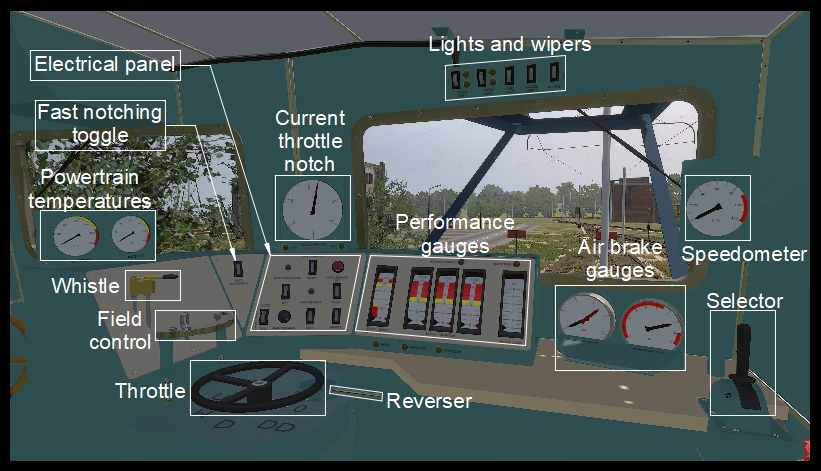
\includegraphics[width=\textwidth]{assets/img-001.png}
\end{center}

\subsubsection{Locomotive performance gauges}
5 locomotive performance gauges are located on a large panel in front of a driver. From left to right these are the voltmeter, 3 traction motor load meters and the total load meter.

The voltmeter is a double-needle gauge. The black hand on the left shows supply voltage, unless rheostatic braking mode (which cuts the entire locomotive from the supply) is enabled. When rheostatic braking is on, the left needle shows the voltage the locomotive blower fans are currently running at. The red hand on the right displays voltage measured at traction motor terminals and is primarily intended to assist a driver with setting up a dynamic brake. It can also be used to judge efficiency of the locomotive -- it's the highest when terminal and supply voltages match; deviation from supply in either direction signifies additional energy losses and reduced efficiency.\footnote{In \powermode{Y} selector mode (see \ref{sec:selector} Selector) the red voltmeter hand is inactive and will always remain at zero due to the way power circuit is set up.}

3 ammeters in the middle show amperages in traction motors No. 1, 3 and 5 respectively. Each meter has 2 hands: black on the left for armature and red on the right for field winding currents.\footnote{The field winding is actually split into 2 halves, and the red hand shows current only in the 2nd half.} The maximum continuous current is 500 A.

The total load meter on the right shows total current drawn by the locomotive from the supply. It includes traction motors and auxiliaries like blowers and compressor. Make sure to keep this gauge below power supply limits at all times, otherwise a power cut may occur.

The yellow ``Reverse current'' lamp at the top middle of the panel indicates that traction motors are working as generators and their armature current is reversed, slowing a train down. It's normal for this lamp to light up in rheostatic or regenerative braking mode.
\newpage

\subsubsection{Pantograph and main breaker panel}
Pantograph and main breaker switches and lamps are located on the slanted electrical panel to the left of a driver. There are 4 pantograph toggle switches, arranged in a cross:
\begin{itemize}
\item Top switch toggles the pantograph on the leading unit,
\item Bottom switch toggles the pantograph on the trailing unit,
\item Right switch extends the trolley on the leading unit for taking power from a right-hand side conductor rail,
\item Left switch extends the trolley on the trailing unit for taking power from a left-hand side conductor rail.
\end{itemize}
The green ``Pantograph air'' light in the top-left corner indicates sufficient air pressure in the control system to raise pantographs and run the locomotive.

Because overhead and side rails run at different voltages, pantographs and trolleys are interlocked to prevent a short circuit. Side trolley cannot be extended with any pantograph up, and pantographs cannot be raised with either trolley pointing outwards.

Like all systems on the locomotive, pantographs are subject to wear and tear. To minimize it:
\begin{itemize}
\item In \powermode{Y} (see \ref{sec:selector} Selector) mode, raise only 1 pantograph,
\item In \powermode{S} and \brakemode{S} modes, raise 2 pantographs at speeds below 20-30 km/h, and 1 above,
\item In \powermode{P} and \brakemode{P} modes, raise 2 pantographs at speeds below 60 km/h, and 1 above, unless current is greater than 500 A. When ammeters are in the red zone, both pantographs should be up at all speeds.
\end{itemize}

The main circuit breaker (MCB) provides overhead power to traction motors and auxiliary systems. To enable MCB, ensure that throttle is at Idle, raise at least 1 pantograph and verify that supply voltage is available, then press the black ``Main breaker on'' button in the bottom-left corner of the panel. The MCB will activate in 2 seconds and the green ``Main breaker'' lamp in the middle of the panel will light up. In rheostatic braking \brakemode{R} mode (see \ref{sec:selector} Selector) the MCB can be toggled on without a power supply.

The MCB will trip automatically if traction motor current exceeds 850 A, or total load goes over 4800 A, or when TM terminal voltage approaches 2000 V, or when all pantographs are retracted and the locomotive is not in rheostatic braking \brakemode{R} mode. It can also be turned off manually by pressing the red ``Main breaker off'' button in the top-right corner of the panel.

\subsubsection{Hand and air brakes}
Each unit of the locomotive has a handbrake stand on the left-hand side of a cab. Both handbrakes should be released prior to moving the locomotive, and at least one should be applied when parking.

The air braking system is charged from 2 large main reservoirs at the bottom of unit A, which are fed by the main compressor located under the nose hood of unit B. The compressor requires at least 1000 V supply to run.

Air brake cab controls include train and independent brake valves and a brake/controls cut-out. The independent brake is a 6 notch straight air brake, which applies shoes on both units of the locomotive. The train brake is a non-self lapping valve with 4 notches: release, lap, application and emergency.

The brake cut-out valve toggles train brake valve and also selects the active cab. It must be turned on for cab controls to function. Shutting off the cut-out will reset all handles and deactivate the cab.

\NB\ Never open brake cut-out in both cabs simultaneously -- only 1 cab should be active at a time.

\Tip\ if it's necessary to control a train brake from another locomotive via a remote, keep brake cut-out active and move train brake handle to ``Lap'' to prevent a conflict.

\subsubsection{Driving handles and related indicators}

\paragraph{Reverser}
The reverser selects movement direction relative to the current cab. It has 3 notches: forward, neutral and reverse, and can be moved by standard reverser keyboard controls (default Y and H).

\paragraph{Throttle, notch dial and fast notching switch}
The throttle wheel in the middle of a control stand controls power and speed of the locomotive by switching resistors in and out of the circuit. Because resistive control is inherently inefficient, the throttle is largely used only for starting and accelerating a train, switching between different motor configurations (see section \ref{sec:selector} Selector) or dynamic braking.

The actual resistors are switched by 2 camshaft controllers: primary and secondary. The primary camshaft, located in unit A, changes resistance in large steps, while the secondary in unit B switches by small amounts for fine control. Each controller has 6 power notches\footnotemark, giving 36 notches in total. \footnotetext{Technically both controllers have 7 notches, however one of them between \#2 and \#3 is a special transitory notch that switches some resistors from series to parallel connection. This notch, marked ``T'' on the dial, gives the same power as \#3 and is always skipped.}

The current position of both camshafts is indicated on a large double needle dial on the top of the control stand. The short black and long red hands correspond to the primary and secondary controllers.

The ``Fast notching'' switch, located on a triangular panel, allows the control system to skip some of the notches when enabled, improving locomotive responsiveness. The yellow lamp on the bottom right corner of the notch display lights up to remind a driver that Fast notching is active.

The bottom-left corner on the notch display houses a red ``Resistance notch'' lamp with a resistor icon next to it. This lamp is lit when the locomotive is running at notch other than \#6 primary / \#6 secondary to remind a driver about a suboptimal running.

The throttle wheel itself has 6 positions:
\begin{enumerate}
\item ``0'' -- Idle. This notch immediately cuts power to traction motors and then runs both camshafts down to \#1. Idling a locomotive when motor current exceeds 250 A will deal varying amount of powertrain damage,
\item ``DD'' -- Run down. If ``Fast notching'' is off, continually runs secondary controller down. Every time it rolls over from \#1 to \#6, the primary is reduced by 1 notch. If ``Fast notching'' is on, runs down both camshafts simultaneously,
\item ``D'' -- Notch down. If ``Fast notching'' is off, drops the secondary by a single notch. Every time it rolls over from \#1 to \#6, the primary notches down. If ``Fast notching'' is on, notches down both camshafts by a single position simultaneously,
\item ``H'' -- Hold. Engages traction motors when throttle was previously at Idle and holds both camshafts at their current notch. A driver must return handle to Hold after using Notch up/down before they can notch up or down again,
\item ``U'' -- Notch up. If ``Fast notching'' is off, advances the secondary by a single notch. Every time it rolls over from \#6 to \#1, the primary notches up. If ``Fast notching'' is on, notches the primary up as long as the secondary is at \#1 and motor current is less than 400 A in \powermode{Y} selector mode (see section \ref{sec:selector} Selector), 300 A in \powermode{S} mode and 250 A in other modes,
\newpage
\item ``UU'' -- Run up. If ``Fast notching'' is off, continually runs the secondary camshaft upwards. Every time it rolls over from \#6 to \#1, the primary notches up. If ``Fast notching'' is on, continually runs the primary up as long as the secondary is at \#1 and motor current is less than 400 A in \powermode{Y} mode, 300 A in \powermode{S} mode and 250 A in other modes.
\end{enumerate}

\danger\ Combining Run up with Fast notching at low speeds can easily lead to over-current, causing main breaker to trip, and possibly damage the locomotive.

The throttle wheel can be operated by standard throttle up/down keyboard controls (default T and G), and Fast Notching -- by dynamic brake keyboard shortcuts (O and L).

Despite being called a throttle, this control is more akin to a clutch in a vehicle with manual transmission.

\paragraph{Selector and Transition light}\label{sec:selector}
The black selector handle is located on the right hand side of a cab and, as its name implies, allows a driver to select between power and dynamic braking modes, as well as choose a motor configuration in either. The currently chosen mode is shown in a small window besides the handle, with power modes represented by a \colorbox{black}{\color{white} white letter on a black background}, and dynamic braking by a \colorbox{red}{black letter on red}.

In a power mode, 2 traction motors on each bogie can connect in either series (selector mode \powermode{S}, half horsepower) or parallel (\powermode{P}, full horsepower). The series mode is used for starting and cruising, while parallel is used for uphill climbing at 30 km/h (20 mph) or faster. A driver can switch between either mode under load as long as throttle is at resistance notch and the red light at the bottom left corner of the notch dial is lit.

\danger\ When going from \powermode{S} to \powermode{P} ensure that motor current is less than 200 A prior to moving the selector to minimize risk of over-current.

For efficient shunting movements within yard limits or for running the locomotive light there is a 3rd \powermode{Y} (1/6 horsepower) mode, which connects all 6 motors in series. Unlike \powermode{S} and \powermode{P}, transitioning from and to \powermode{Y} mode can only be done with throttle at Idle.

Dynamic braking modes include rheostatic \brakemode{R}, regenerative in parallel \brakemode{P} and regenerative in series \brakemode{S}. The rheostatic braking is always done in parallel, doesn't require external power nor being on an electrified track, is usable at any speed and can bring a train to an almost complete stop. The regenerative braking, on the other hand, is more powerful and allows to recover energy and save electricity, but is power supply dependent and its speed range is limited. The series regenerative mode is effective between 30 and 60 km/h, while parallel regen has a minimum speed of 65 km/h. Changing among all dynamic brake modes requires throttle at Idle.

The keyboard controls for the selector are standard Gearbox A shortcuts (default [ and ').

The red Transition lamp at the top right corner of the control stand indicates that selector contactors are moving and transition has not yet been completed.

While the selector might resemble a gearbox in a manual car at the first glance, it actually controls horsepower of a locomotive, acting more like a gas pedal.
\newpage

\paragraph{Field control handle}
Field control handle, located on the left-hand side of the control stand, selects the amount of field weakening in power and rheostatic braking modes and directly controls field current in both regenerative modes. It has 13 notches (R1-R13), however weak field only uses first 7, which are also named FF, WF1-WF6; the remaining R8-R13 notches are exclusively for regen.

The field shunt ratios are as follows: 100\% at FF/R1, 85\% at WF1/R2, 80\% at WF2/R3, 75\% at WF3/R4, 40\% at WF4/R5, 35\% at WF5/R6 and 30\% at WF6/R7. In regenerative mode, the field current ranges from 100 A at FF/R1 to 330 A at R13.\footnote{Due to the inner workings of regen, the actual current range varies with voltage, speed and load of motors.}

The standard Gearbox B keys (default ] and \textbackslash) are used to move the field control handle.

\danger\ When running in parallel \powermode{P} mode do not use field weakening notches WF3-WF6 unless speed is 70 km/h or faster.

The field control handle is what closely corresponds to a gearbox in a manual transmission, though unlike in a mechanical one, there are no upper speed limits for ``gears''. Also the ``gear ratios'' can change with speed, due to the influence of magnetic flux inside motors being fully saturated above 300 A.

\paragraph{Handle interlocks}
To minimize risk of damage, some handles are interlocked and can only be moved under certain conditions.

The reverser can be moved only with throttle at idle. Conversely, moving throttle away from idle is only possible when reverser is not in neutral.

The selector can be moved between \powermode{S} to \powermode{P} as long as throttle is at resistance notch and the red light at the bottom left corner of the notch dial is lit. Switching to or from other modes requires throttle at Idle.

Unlike throttle and reverser, selector is not interlocked mechanically. Instead, when disallowed movement is made, the transition lamp will begin to flash accompanied by a warning buzzer and the actual selector won't switch until the buzzer is canceled. To cancel the buzzer, either return the selector handle to the position where it originally was, or idle the throttle.

Field handle is not interlocked and can be moved freely as long as brake/controls cut-out is in.

\subsubsection{Miscellaneous controls, gauges and signal lamps}
The sander toggle switch is located at the bottom right corner of the slanted panel. The sander is non-adjustable and can only be toggled on and off. When sanders are active, the yellow Sand lamp at the bottom of the main panel is lit.

\note\ Unlike vanilla locomotives, there is no sand gauge, though there is red Low Sand warning light.

The cooling blower control switch is found in the bottom-left corner of the slanted electrical panel. It toggles between Automatic and Full speed modes. In automatic mode, cooler fans switch on at low speed when reverser is not in neutral. They go to full speed once motor current exceeds 350 A and revert back to low once current drops below 250 A. When reverser is returned to neutral, blowers shut down. In full speed mode, blowers run continually at full speed regardless of the reverser and current.\footnote{To provide adequate cooling in a wide range of supply voltages, the locomotive is equipped with 6 separate blowers driven by 1000 V motors. When supply voltage is in 900-1500 V range, blower motors connect either in 2 parallel groups of 3 (low speed) or 3 groups of 2 (high speed). At a reduced (600-900 V) voltage blowers instead switch between either 3 groups of 2 (low speed) or full parallel (high speed).}

When locomotive is running in rheostatic braking \brakemode{R} mode, blowers are directly and fully powered by traction motors and fan control switch has no effect.\footnote{In rheostatic braking mode, 2 motors on a bogie power 2 blowers which work in parallel when motor voltage is 900 V or less, and switch to series whenever voltage goes over 950 V.}

The small box on the top of the control stand above the field control handle houses 2 thermometers. The left measures temperature in starting/braking resistances, the right -- in traction motors.
A brass whistle handle is also located above the field control.

Above right-hand side window there is an overhead lighting and wipers control panel with 5 toggles. From left to right these are:
\begin{enumerate}
\item Headlights -- off, dim and bright. 2 lamps next to the switch indicate brightness: no lamps for off, one lamp for dim, both lamps for bright,
\item Ditch lights -- off, red and white, shown by 2 small lights next to the switch,
\item Cab light -- simple toggle, no brightness adjustment,
\item Gauge lights -- simple toggle,
\item Wipers -- off, intermittent, continuous.
\end{enumerate}
\note\ switches on the lighting panel are not communicated between units and must be set separately.
\newpage

\section{Driving Checklists}

\subsection{Preparing a locomotive}
To get the locomotive ready, perform the following steps:
\begin{enumerate}
\item Go to machinery room on unit B,
\item Open the battery panel,
\item Enable ``Electrics'' knife switch. Leave the nearby ``Jog'' switch off,
\item If pressure in the control air reservoir is below 4 bar, the auxiliary compressor will automatically start.
\item Make sure that the locomotive is on an electrified track. If it isn't, use Jogging mode (see section \ref{sec:jogging}) or another locomotive to bring it to powered rail section,
\item Verify that control air is at least 3 bar and open ``Pantograph air'' valve,
\item Go to a cab where the locomotive will be driven from and open air brake cut-out to activate it and unlock the controls,
\item Toggle ditch and/or headlight switches in both cabs as required,
\item Verify that the green ``Pantograph air'' lamp is lit and throttle wheel is at Idle, and raise pantograph or extend a side trolley as appropriate,
\item Wait until voltmeter registers a power supply,
\item Press ``Main breaker on'' button to enable the MCB. The green ``Main breaker'' lamp will light up after 2 seconds. If the main reservoir pressure is low and supply voltage is at least 1000 V, the main air compressor will automatically start,
\item Ensure or wait until main reservoirs are at least at 5.5 bar and fully apply the independent brake,
\item Release the train brake to charge the brake pipe,
\item Release handbrakes in both cabs. The locomotive is now fully operational.
\end{enumerate}

\subsection{Starting movement}
To get a train moving, perform the following steps:
\begin{enumerate}
\item Set the reverser to the desired direction and field handle to FF/R1,
\item Move selector to \powermode{S},
\item Move throttle to ``H'' and wait for motor current to register,
\item Release air brakes. The train will begin to move,
\item Advance throttle all the way to \#6 primary / \#6 secondary either manually by alternating between ``U'' and ``H'' or continually by using ``UU''. Motor current should be kept as high as adhesion and temperature permit to minimise resistive losses. Fast notching mode can be used to speed up acceleration with a light consist,
\item Once both camshafts are at \#6, accelerate further or control speed using field handle for as long as practical before switching to parallel. Unlike the throttle, field weakening doesn't incur additional energy losses.
\end{enumerate}
\Tip\ If the track ahead is flat or downhill, it's more efficient to accelerate in \powermode{Y} mode first and switch to \powermode{S} after speed reaches 20 km/h.

\subsection{Upshifting from \powermode{S} to \powermode{P}}
To transition from series to parallel safely, perform the following steps:
\begin{enumerate}
\item Return field handle to FF/R1,
\item Throttle down at least once and until current is at less than 200 A to minimise risk of overcurrent,
\item Move the selector from \powermode{S} to \powermode{P} and wait 2-3 seconds for transition to complete,
\item Accelerate the train by advancing the throttle all the way to \#6 primary / \#6 secondary, keeping the current as high as track conditions, temperature and power supply limits permit,
\item Once both camshafts are at \#6, control speed using field handle or downshift back to series when cruising on a level track.
\end{enumerate}

\subsection{Downshifting from \powermode{P} to \powermode{S}}
Going back to series from parallel is safe at any speed and involves the following steps:
\begin{enumerate}
\item Return field handle to FF/R1,
\item Disable fast notching if it's on,
\item Throttle down to \#6 primary / \#5 secondary,
\item Move the selector from \powermode{P} to \powermode{S} and wait 2-3 seconds for transition to complete,
\item Notch up to return secondary camshaft to \#6,
\item Control speed using field handle.
\end{enumerate}

\subsection{Coasting}
To minimise powertrain wear and tear, shutting off power should be done as follows:
\begin{enumerate}
\item Enable fast notching,
\item Move throttle to ``DD'',
\item Wait until both camshafts stop at \#1,
\item Move throttle to Idle.
\end{enumerate}

\subsection{Shunting}
Shunting is typically performed in \powermode{Y} mode at low speeds and involves frequent stops and reversals. Because the risk of overcurrent in \powermode{Y} mode is minimal, the following procedure is recommended to keep flat switching resistance losses small:
\begin{enumerate}
\item Set the reverser to the desired direction,
\item Move selector to \powermode{Y},
\item Enable Fast notching mode,
\item Release air brakes.
\item Move throttle to ``H'' and wait for motor current to register. The train will begin to move,
\item Immediately move throttle to ``UU'' to accelerate as fast as camshafts permit. Apply sand if necessary,
\item Once both camshafts reach \#6, control speed with the field handle.
\end{enumerate}

\subsection{Shutdown}
To shut down the locomotive:
\begin{enumerate}
\item Apply handbrakes,
\item Close the brake cut-out. This will automatically disengage the MCB and retract all pantographs,
\item Switch head and ditch lights off,
\item Go to the battery panel in machinery room of unit B, close ``Pantograph air'' valve and turn off ``Electrics'' knife switch.
\end{enumerate}

\subsection{Cab change}
To change cabs, apply emergency brake and close the brake cut-out to disengage the MCB and retract all pantographs. Then go to the other cab and open the brake cut-out to activate it. Afterwards perform steps 9-13 from checklist 4.1 to restart the locomotive.

\subsection{Jogging}\label{sec:jogging}
Jogging is a special movement mode that uses onboard battery power to move the locomotive on a flat track at 3-7 km/h where overhead power is not available, e.g. turntables and service sheds. To activate jogging, perform the following steps:
\begin{enumerate}
\item Ensure that the ``Electrics'' knife switch is on, ``Pantograph air'' is open, pressure in the control tank is at least 3 bar and one of the cabs is activated,
\item Set the reverser to the desired direction,
\item Set the selector to \powermode{Y} for precision or \powermode{S} for faster movement,
\item Release/vent all air and handbrakes,
\item Go to the battery panel in machinery room of unit B,
\item Close the ``Pantograph air'' valve and turn ``Electrics'' knife switch off. This is a safety interlock to ensure that the battery won't end up under full catenary voltage,
\item Enable ``Jog'' knife switch on the right side of the panel. The locomotive will immediately begin to move in the direction selected in step 2 as long as the track isn't too inclined,
\item To end the jogging mode, turn ``Jog'' knife switch off and re-enable ``Electrics'' and ``Pantograph air''.
\item Apply an air or hand brake to stop.
\end{enumerate}

\caution\ Because jogging requires ``Electrics'' to be off, none of the locomotive appliances, including lights and powered gadgets will work in jogging mode, and cab controls, except hand and air brakes, will no longer respond. Make sure to bring enough flashlights and lanterns to illuminate the interior and outside of the locomotive when jogging at night.
\newpage

\section{Dynamic braking checklists}

\subsection{Rheostatic braking}
To engage the rheostatic brake, perform the following steps:
\begin{enumerate}
\item Ensure that the MCB is toggled on, throttle is at Idle and the reverser direction matches movement,
\item Move selector to \brakemode{R}. The voltmeter will drop down to zero,
\item If speed is 50 km/h or faster, move field handle to WF3/R4\\
\danger\ Skipping this step at high speed may cause motor voltage to spike over 2000 V and damage the locomotive,
\item Move throttle to ``H''. The primary camshaft will advance to notch \#3, which is the minimum notch for usable braking force,
\item At 45 km/h or higher, motors will energize immediately and braking will commence. Lower speeds may require throttling further up to ``wake up'' the motors. Advance throttle gradually and be prepared to notch down once or twice to ``catch'' the rising current,
\item Once the current stabilizes, control braking force with the field handle at 50 km/h or higher, or with the throttle at lower speeds. Keep an eye on motor voltage and do not allow it climb over 2000 volts.
\end{enumerate}

\caution\ The maximum power the resistors can dissipate continually is 3 MW, while traction motors are capable of generating more than 4 MW. Monitor resistor temperature gauge closely and reduce current if it starts to approach the red line.

\caution\ Traction motors can't generate sufficient power to keep cooler blowers running at speeds less than 25 km/h. Riding the rheostatic brake at such low speeds with high currents for an extended period of time will eventually overheat the motors.

\caution\ Because rheostatic brake cuts the power supply entirely, the compressor will not function. Avoid repeated train brake applications and releases in rheostatic mode.

\Tip\ To set up rheostatic brake at low speeds quickly, enable Fast notching and advance primary camshaft to \#6 at less than 10 km/h, \#5 at 10-20 km/h and \#4 at 20-35 km/h.

\Tip\ To maximise cooling efficacy, combine throttle and field weakening to keep the black needle on the voltmeter in 800-900 V range. Increasing field weakening reduces both motor amperage and voltage, while throttling down also reduces motor amperage but raises voltage-to-current ratio.
\newpage

\subsection{Regenerative braking}
The regenerative brake set-up is more involved and carries more hazards compared to rheostatic:
\begin{enumerate}
\item Ensure that the overhead power voltage is at least 1200 V, the MCB is toggled on, throttle is at Idle, field control handle is at FF/R1 and the reverser direction matches movement\\
\danger\ Neglecting to return the field handle to FF/R1 may damage the locomotive during setup,
\item Set the selector handle to \brakemode{S} if speed is between 30 and 60 km/h, or \brakemode{P} if speed is above 65 km/h\\
\danger\ Selecting an incorrect range may damage the locomotive during later stages of set-up,
\item Move throtle to ``DD'' to spool up cooling blowers and an auxiliary generator under the nose hood of unit A, which will supply power to the field windings. Wait for field currents and motor terminal voltage to settle,
\item Gradually push the field handle forward until TM terminal voltage matches or slightly exceeds the supply,
\item Move throttle to ``H'' to fully engage traction motors. The armature ammeters will show current, and the ``Reverse current'' lamp will light up. If the lamp remains dark, move the field handle further forward until it turns on,
\item Notch / run the throttle up all the way to \#6 primary / \#6 secondary while keeping an eye on TM terminal voltage. Adjust the field handle as necessary to keep TM voltage no higher than 100-200 V above the supply.\\
\danger\ Letting TM voltage to climb over 2000 V will damage the locomotive,
\item Once throttle is at \#6 primary / \#6 secondary, control braking force and speed with the field handle.\\
\danger\ Avoid moving the handle in big steps. Traction motors are very sensitive to field changes during regen and can over-current or revert back to motoring easily.
\end{enumerate}

Disengaging the regenerative brake properly also requires a special procedure:
\begin{enumerate}
\item Enable Fast notching,
\item Gradually retract the field handle until armature current is below 250 A and preferably as close to zero as possible,
\item Move throttle to ``DD'' and wait until both camshafts reach \#1. Keep an eye on TM terminal voltage and adjust the field handle to keep it no more than than 100-200 V above the supply\\
\danger\ Letting TM voltage to go over 2000 V will damage the locomotive,
\item Idle the throttle to disconnect traction motors and shut down the auxiliary generator,
\item Return the field handle to FF/R1.
\end{enumerate}

\danger\ Regenerative brake should never be left active under a neutral section. Doing so will damage the locomotive.

\danger\ In regenerative mode, grid load limits still apply. Do not exceed the maximum prescribed current on the Total load gauge. A sudden power cut will cause arcing and damage the locomotive.

\Tip\ By using upper resistance notches a driver can boost the field current while keeping armature within limits and thus obtain greater braking force at the expense of reduced energy recovery. However, it's still important not to allow TM voltage to go over 2000 V, otherwise a breaker will trip and the locomotive will receive damage.

\Tip\ While intended for braking, it's also possible to utilise regen for traction by setting the field in such a way that TM terminal voltage is below supply. This can be useful when going over an undulating track profile, as it allows to shift from power to braking and back quickly. Driving around in regen is slightly less efficient compared to a regular power mode because of the need to keep auxiliary field generator running, which may consume up to 200 kW. In addition, it's not possible to shift between series and parallel under load -- changing the regen configuration requires fully idling the locomotive.

\Tip\ Another situation where ``regen-as-power'' may be useful are long uphill climbs, where the locomotive may be temperature-limited. The auxiliary generator restricts the field current to no more than 330 A, which drastically reduces the amount of heat emitted inside, while still letting motors deliver their full torque with higher currents for a longer period of time.

\section{Power grid coverage and load limits}

There are 7 operational sections of overhead contact system (OCS) on the map:
\begin{itemize}
\item The SM district with an OWC-FM-SM branch, the northbound route extending to FF/OWN and the south-east road to HB,
\item The FF district with branches leading to SM and OR, and 2 lines extending towards IMW and IME/CME,
\item The IME/CME district, which includes both mines in the eastern portion of the map and runs until the ``big tunnel loop'' on the northern part,
\item The IMW line which bridges CP and FF. IMW storage yard itself is not electrified,
\item The CP yard,
\item The OR yard,
\item The HB yard and the mainline from HB towards SM. Storage (S) sidings and the entire container terminal (D yard) do not have catenary and are not planned to receive electrification.
\end{itemize}

All districts run at 1500 V DC, with the exception of CP and OR yards where the voltage is only 750 V due to clearances. Some sidings in SM and IME yards use side-mounted rail to provide power. All side rails run at 1000 V.\footnote{The actual output voltage is 10 \% higher to compensate for drops. The exceptions are SM district and OR yard where the voltages are exactly 1500 V and 750 V respectively.}

The standard grid current limit is 4000 A, excluding IME/CME district (where the maximum current has been raised to 5500 A to allow heavy trains to negotiate long steep inclines) and the OR yard. The current limit for OR and side rails in IME and SM is 2000 A.

\NB\ It's forbidden to use \powermode{P} parallel mode within OR yard limits.

If a grid limit is exceeded, there is a chance that a breaker at the substation will trip and cut the power out. The electricity is automatically restored after 10 seconds; however if there was another outage in the last 5 minutes, then the downtime will be extended to 30 seconds.
\newpage

\section{Signage}

A few areas of electrified track require a driver to shut off power and coast. These areas a marked with one of the following signs. Unlike regular speed posts, these signs are not always located on the right-hand side of a track.

\renewcommand{\arraystretch}{1.35}
\begin{tabular}{@{}m{22mm}m{145mm}@{}}
\centering
\includegraphics[width=13mm]{assets/img-002.png} & This sign warns about approaching a neutral section -- a portion of OCS which is normally dead and whose purpose is to electrically insulate different subdivisions of the catenary. A driver must prepare to shut off power or regenerative brake before entering the neutral section.\\
\centering
\includegraphics[width=13mm]{assets/img-003.png} & This sign marks the beginning of a neutral section. Throttle must be brought to Idle and the main breaker turned off before passing this sign.\newline 
\note\ The rheostatic brake always fully disconnects the locomotive from the catenary and is completely safe to use under a neutral section.\\
\centering
\includegraphics[width=13mm]{assets/img-004.png} & This sign marks the end of a neutral section. A driver can re-enable the main breaker and reapply power after the front of the locomotive having passed this sign and verifying that the voltmeter shows proper supply voltage.\\
\centering
\includegraphics[width=13mm]{assets/img-005.png} & This sign marks the end of a neutral section, but also warns a driver that a track ahead runs at reduced (less than 1000 V) voltage, where some of the locomotive systems will not function. A driver can re-enable the main breaker and reapply power after the front of the locomotive having passed this sign and verifying that the voltmeter shows proper supply voltage.\\
\centering
\includegraphics[width=13mm]{assets/img-006.png} & This sign warns about approaching a termination or a physical gap in an overhead line. A driver must prepare to either stop or shut off the power or regenerative brake and lower all pantographs before the line ends.\\
\centering
\includegraphics[width=13mm]{assets/img-007.png} & This sign marks the end of a usable catenary. A driver must either not overrun this sign or lower both pantographs when passing it.\\
\centering
\includegraphics[width=13mm]{assets/img-008.png} & This sign marks the beginning of a usable catenary. A driver may raise pantographs and reapply power after the entire locomotive has passed this sign.\\
\end{tabular}

\newpage
\appendix
\section{HUD changes}

The meaning of some HUD controls has been changed from vanilla game:
\begin{itemize}
\item Gearbox A corresponds to selector. Y, S and P are respective power modes, R is rheostatic brake, RGS and RGP are series and parallel regenerative,
\item Gearbox B is the field handle. FF means ``Full field'' (maximum torque, low speed), ``WFx'' -- weakened field (smaller torque, higher speed), ``Rx'' -- regenerative brake notch,
\item The ``Power'' readout is actually the throttle notch display. The first digit is the primary notch, the 2nd -- secondary. For example, number ``35'' denotes \#3 primary / \#5 secondary throttle,
\item The ``Dynamic Brake'' represents the Fast Notching switch. 0 \% is off, 100 \% is on.
\end{itemize}

\section{Operation with damaged traction motor(s)}

When traction motor(s) are damaged and cut-out, the locomotive operation changes as follows:
\begin{itemize}
\item The \powermode{Y} mode becomes unusable,
\item In \powermode{S}, \brakemode{S} and \brakemode{R} modes both the defective motor and another motor on the same bogie are cut out,
\item In \powermode{P} and \brakemode{P} modes only the defective motor is cut out.
\end{itemize}

\end{document}
